\documentclass[a4paper]{article}

\usepackage{pgfplots}

\usepgfplotslibrary{patchplots}
\pgfplotsset{compat=1.6}

\begin{document}

%\tracingmacros=2 \tracingcommands=2

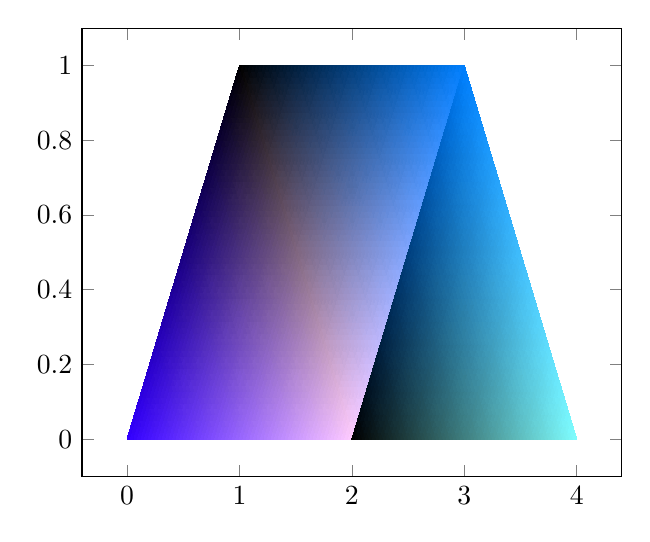
\begin{tikzpicture}
    \begin{axis}
    \addplot[
		patch,
		table/row sep=\\,
		mesh/color input=explicit,
		shader=interp,
		point meta/symbolic={\thisrow{R},\thisrow{G},\thisrow{B}},
		patch table={%
			0 1 2\\
			1 2 3\\
			4 3 5\\
		}]
    table[row sep=\\]
	{
        x y R G B \\
        0 0 0.2 0 1\\% 0
        1 1 0 0 0\\% 1
        2 0 1 0.8 1\\% 2
        3 1 0 0.5 1\\% 3
        2 0 0 0 0\\% 4
        4 0 0.5 1 1\\% 5
    };
    \end{axis}
\end{tikzpicture}

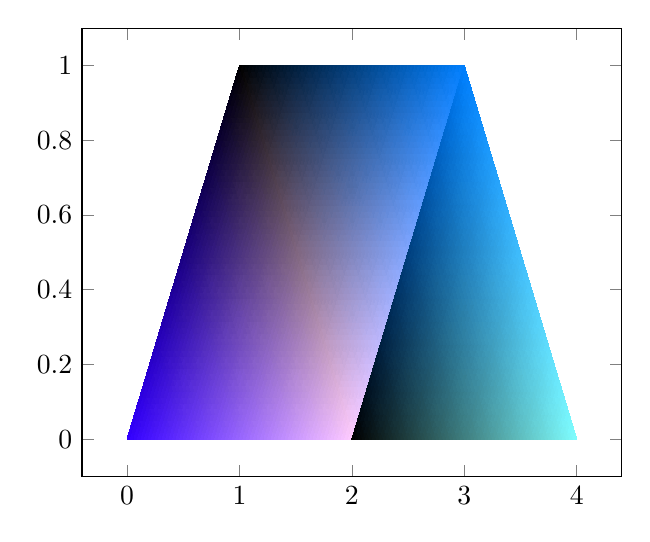
\begin{tikzpicture}
    \begin{axis}
    \addplot[
		patch,
		table/row sep=\\,
		mesh/color input=explicit,
		shader=interp,
		point meta/symbolic={\thisrow{R},\thisrow{G},\thisrow{B}},
	]
    table[row sep=\\]
	{
        x y R G B \\
        0 0 0.2 0 1\\% 0
        1 1 0 0 0\\% 1
        2 0 1 0.8 1\\% 2
%
        1 1 0 0 0\\% 1
        2 0 1 0.8 1\\% 2
        3 1 0 0.5 1\\% 3
%
        2 0 0 0 0\\% 4
        3 1 0 0.5 1\\% 3
        4 0 0.5 1 1\\% 5
    };
    \end{axis}
\end{tikzpicture}

\end{document}

